
Given a parallelogram ABCD we have to prove that
\begin{figure}[!ht]
	\centering
	\resizebox{\columnwidth}{!}{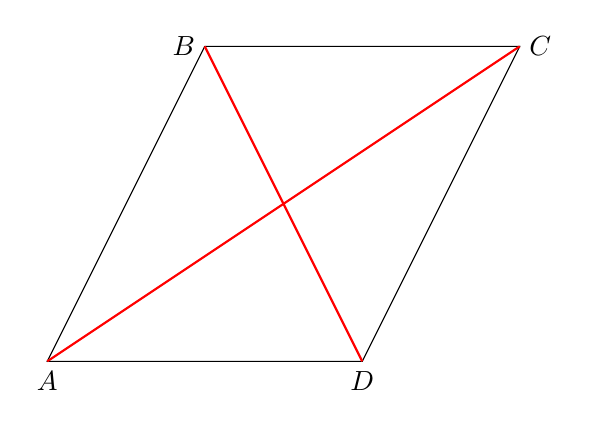
\begin{tikzpicture}	
	\draw (0,0) node[anchor=north]{$A$}
	-- (2,4) node[anchor=east]{$B$}
	-- (6,4) node[anchor=west]{$C$}
	-- (4,0) node[anchor=north]{$D$}
	-- cycle;
	\draw[red][thick] (2,4) -- (4,0) 	-- cycle;
	\draw[red][thick] (6,4) -- (0,0) 	-- cycle;
\end{tikzpicture}}
	\caption{parallelogram ${ABCD}$}
	\label{eq:solutions/1/101/fig1:Parallelogram}
\end{figure}
	
\begin{align}\label{eq:solutions/1/101/eq:1}
    	\norm{\vec{A-C}}^2 + \norm{\vec{B-D}}^2 = \nonumber  \norm{\vec{A-B}}^2+\norm{\vec{B-C}}^2+\\\norm{\vec{D-C}}^2+\norm{\vec{A-D}}^2
\end{align}

 The diagonals of  parallelogram are
\begin{align}
	\vec{A-C} = (\vec{A-D}) +(\vec{D-C})\\
	\vec{B-D} = (\vec{A-D}) -(\vec{A-B})
\end{align} 
The sum  of the squares of diagonals is
\begin{align}
\norm{\vec{A-C}}^2 +\norm{\vec{B-D}}^2 = \nonumber  
\norm{(\vec{A-D}) +(\vec{D-C})}^2\\+ \norm{(\vec{A-D}) -(\vec{A-B})}^2
\end{align}
\begin{align}
=\norm{\vec{A-D}}^2 +\norm{\vec{D-C}}^2 + 2{(\vec{A-D})}^T{(\vec{D-C})} + \nonumber 
\\\norm{\vec{A-D}}^2+\norm{\vec{A-B}}^2-2{(\vec{A-D})}^T{(\vec{A-B})}\label{eq:solutions/1/101/eq:2}
\end{align}

\begin{align}\label{eq:solutions/1/101/eq:3}
= \norm{\vec{A-D}}^2 +\norm{\vec{D-C}}^2 + 2\norm{\vec{A-D}}\norm{\vec{D-C}}\nonumber 
\\\cos(180\degree-\angle{ADC})  +\norm{\vec{A-D}}^2+\norm{\vec{A-B}}^2\nonumber 
\\-2{\norm{\vec{A-D}}\norm{\vec{A-B}}}\cos\angle{DAB}
\end{align}
In the parallelogram $ABCD$  
\begin{align}
	\norm{\vec{A-D}}&=\norm{\vec{B-C}}\label{eq:solutions/1/101/eq:4}\\
	\norm{\vec{A-B}} &= \norm{\vec{D-C}}\label{eq:solutions/1/101/eq:5}\\
	\angle{ADC} + \angle{DAB} &= 180\degree\\
	\angle{DAB} &= 180\degree -\angle{ADC} \label{eq:solutions/1/101/eq:6}
\end{align}
From equation \eqref{eq:solutions/1/101/eq:3},\eqref{eq:solutions/1/101/eq:4},\eqref{eq:solutions/1/101/eq:5}  and \eqref{eq:solutions/1/101/eq:6}
\begin{align}
=\norm{\vec{B-C}}^2 +\norm{\vec{D-C}}^2+2\norm{\vec{A-D}}\norm{\vec{A-B}}\cos\nonumber\\\angle{DAB}+ \norm{\vec{A-D}}^2+\norm{\vec{A-B}}^2-2{\norm{\vec{A-D}}\norm{\vec{A-B}}}\nonumber\\\cos\angle{DAB}\label{eq:solutions/1/101/eq:7}  
\end{align}

Simplifying equation \eqref{eq:solutions/1/101/eq:7}
\begin{align}
   \norm{\vec{A-C}}^2 + \norm{\vec{B-D}}^2 = \nonumber  \norm{\vec{A-B}}^2+\norm{\vec{B-C}}^2+\\\norm{\vec{D-C}}^2+\norm{\vec{A-D}}^2\label{eq:solutions/1/101/eq:8}
\end{align}

The equations \eqref{eq:solutions/1/101/eq:1}  and \eqref{eq:solutions/1/101/eq:8} are equal,hence proved
